% SVN info for this file
\svnidlong
{$HeadURL$}
{$LastChangedDate$}
{$LastChangedRevision$}
{$LastChangedBy$}

\chapter{Omotopia}
\labelChapter{omotopia}

\begin{introduction}
	‘‘BEEP BOOP INSERIRE CITAZIONE QUA BEEP BOOP.''
	\begin{flushright}
		\textsc{NON UN ROBOT,} UN UMANO IN CARNE ED OSSA BEEP BOOP.
	\end{flushright}
\end{introduction}
% citazione
\noindent Finora abbiamo visto omeomorfismi tra spazi topologici sotto tanti aspetti diversi, definendo rigorosamente quella che era l'intuizione del magico materiale elastico. Possiamo osservare tuttavia delle ‘‘\textit{equivalenze di forma}'' che un omeomorfismo è troppo rigido per descriverle.\\
Ad esempio, si possono considerare \textit{equivalenti} figure con lo stesso numero di buchi. Sotto questo punto di vista, la figura corrispondente alla lettera \textsf{\textbf{O}} e quella corrispondente a \textsf{\textbf{P}} sono \textit{equivalenti}, dato che hanno entrambe un solo buco, mentre \textsf{\textbf{X}} non lo è perché non ne ha. Allo stesso tempo, nessuna di queste è \textit{omeomorfa} all'altra: infatti, se togliamo dalle tre lettera/figure un punto come il nodo di raccordo delle ‘‘stanghette'' (o per \textsf{\textbf{O}} un punto qualunque), otteniamo per \textsf{\textbf{O}} una componente connessa, per \textsf{\textbf{P}} due e per \textsf{\textbf{X}} ben quattro distinte.\\
Preceduto da un'approfondimento delle componenti connesse (anche per archi), nel presente capitolo formalizzeremo questo tipo di equivalenza più debole e allo stesso tempo più ampia: l'\textbf{omotopia}.
\section{Lemma di incollamento}
\begin{lemming}\textsc{Lemma di incollamento}\label{lemmaincollamento}\\
	Siano $X,\ Y$ spazi topologici e $X=A\cup B$. Siano $\funz{f}{A}{Y}$ e $\funz{g}{B}{Y}$ continue tali che $f\left(x\right)=g\left(x\right)\ \forall x\in A\cap B$, cioè $f_{\mid A\cap B}=g_{\mid A\cap B}$.\\
	Consideriamo l'\textbf{incollamento}\index{incollamento} $\funz{h}{X}{Y}$ definito da:
	\begin{equation}
		h\left(x\right)=\begin{cases}
			f\left(x\right)\ x\in A\\
			g\left(x\right)\ x\in B
		\end{cases}
	\end{equation}
	Se $A$ e $B$ sono entrambi aperti in $X$ (o entrambi chiusi in $X$), allora $h$ è continua.
\end{lemming}
\begin{demonstration}
	Supponiamo $A$ e $B$ aperti. Sia $U\subseteq Y$ aperto. Allora:
	\begin{equation*}
		h^{-1}\left(U\right)=\underbrace{f^{-1}\left(U\right)}_{\subseteq B}\cap \underbrace{g^{-1}\left(U\right)}_{\subseteq B}
	\end{equation*}
Essendo $f,\ g$ continue, segue che $f^{-1}\left(U\right)$ è aperto in $A$ e $g^{-1}\left(U\right)$ è aperto in $B$.\\
In quanto $A,\ B$ aperti, per definizione di aperto del sottospazio\footnote{Poichè un aperto del sottospazio è dato dall'intersezione del sottospazio con un aperto di $X$, se abbiamo che anche il sottospazio è aperto di $X$, l'intersezione è aperta: in questo caso ogni aperto del sottospazio è anche aperto di $X$.} $f^{-1}\left(U\right)$ e $g^{-1}\left(U\right)$ sono aperti su $X\implies h^{-1}\left(U\right)$ aperto.\\
Il caso di $A$ e $B$ chiuso è esattamente analogo. 
\end{demonstration}
\section{Componenti connesse e componenti c.p.a.}
Riprendiamo la trattazione delle componenti connesse e \textbf{c.p.a.} introdotte nel \autoref{chap:Connessocompatto}.
\begin{define}\textsc{Componente connessa.}\\
	Una \textbf{componente connessa}\index{componente!connessa} di $X$ spazio topologico è uno spazio $C\subseteq X$ \textit{connesso} \textbf{massimale}, tale per cui:
	\begin{equation}
		C\subseteq A\subseteq X\text{ con }A\text{ connesso}\implies C=A 
	\end{equation}
\vspace{-6mm}
\end{define}
\begin{observes}~{}
\begin{itemize}
	\item Le componenti connesse formano una \textit{partizione} di $X$.
	\item Se $x\in X$ si può definire la componente connessa che contiene $x$:
	\begin{equation}
		C\left(x\right)=\union\left\{C\subseteq X\mid x\in C,\ C\text{ connesso}\right\}
	\end{equation}
\item Le componenti connesse possono essere viste come classi di equivalenza per la seguente relazione di equivalenza su $ X $:
	\begin{equation}
		x,\ y\in X\qquad x\sim_C y\iff \exists C\subseteq X\text{ connesso}\ \colon x,\ y\in C
	\end{equation}
\end{itemize}
\vspace{-6mm}
\end{observes}
\begin{demonstration}
Innanzitutto mostriamo che la relazione è di equivalenza:
\begin{itemize}
\item \textsc{Riflessiva}: $x\sim_C x$ è vero, dato che $\left\{x\right\}$ è sempre un connesso.
\item \textsc{Simmetrica}: ovvia dalla definizione.
\item \textsc{Transitiva}: Supponiamo $x\sim_C y,\ y\sim_C z$. Allora $\exists C,\ D\subseteq X$ connessi tale che $x,\ y\in C$ e $y,\ z\in D$. Allora $C\cup D$ contiene sia $x$ che $z$. Inoltre, essendo $y\in C\cap D\implies C\cap D\neq \emptyset$, dunque $C\cup D$ è un connesso: vale $x\sim_C z$.\\
Mostriamo che le classi di equivalenza sono le componenti connesse per $x$.\\
$\includedx$ Se $C\subseteq X$ è una componente connessa, allora $\forall x, y\in C$ si ha $x\sim_C y$, cioè $C$ è interamente contenuta in $C_0=[x]=[y]$ classe di equivalenza per $\sim_C$: $C\subseteq C_0$.\\
$\includesx$ Sia $z\in C_0$ classe di equivalenza e sia $x\in C$ componente connessa. Allora: $x\sim_C z\implies \exists T\subseteq X \text{ connesso}\ \colon x,\ z\in T$.\\
Consideriamo $C\cup T$. $C$ e $T$ sono connessi, $x\in C\cap T\implies C\cap T\neq \emptyset$: $C\cup T$ è ancora connessa. In quanto $C$ è componente connessa, poiché $C\subseteq C\cup T$, per definizione segue che $C=C\cup T$, cioè $T\subseteq C$. Allora $z\in C$ e $C_0\subseteq C$.
\end{itemize}
\vspace{-3mm}
\end{demonstration}
\begin{define}\textsc{Componente c.p.a..}\\
Una \textbf{componente c.p.a.}\index{componente!c.p.a.} di $X$ è una classe di equivalenza per la relazione $\sim_A$ così definita:
	\begin{equation}
	x,\ y\in X\qquad x\sim_A y\iff \exists \alpha\textsc{ cammino in }X\ \colon \alpha\left(0\right)=x,\ \alpha\left(1\right)=y
\end{equation}
\vspace{-6mm}
\end{define}
\begin{demonstration}
	Mostriamo che sia una relazione di equivalenza:
	\begin{itemize}
		\item \textsc{Riflessiva}: $x\sim_A x$ è vero, dato che esiste sempre il \textbf{cammino costante}\index{cammino!costante} nel punto $x$: \begin{equation}
			\funztot{c_x}{I}{X}{t}{x}
		\end{equation}
		\item \textsc{Simmetrica}: se $x\sim_A y$ sappiamo che $\exists\ \funz{\alpha}{I}{X}$ tale per cui $\alpha\left(0\right)=x,\ \alpha\left(1\right)=y$. Possiamo definire il \textbf{cammino inverso}\index{cammino!inverso}:
		\begin{equation}
			\funztot{\overline{\alpha}}{I}{X}{t}{\alpha\left(1-t\right)}
		\end{equation}
	\begin{itemize}
		\item $\overline{\alpha}$ è continuo, perché composizione di applicazioni continue:\\
		\begin{center}
			\begin{tikzcd}
				I \arrow[r]          & I \arrow[r, "\alpha"]  & X                      \\[-25pt]
				t \arrow[r, maps to] & 1+t \arrow[r, maps to] & \alpha\left(1-t\right)
			\end{tikzcd}
		\end{center}
	\item $\overline{\alpha}\left(0\right)=\alpha\left(1\right)=y,\ \overline{\alpha}\left(1\right)=\alpha\left(0\right)=x$.
	\end{itemize}
Allora il cammino $\overline{\alpha}$ definisce $y\sim_A x$.
		\item \textsc{Transitiva}: Supponiamo $x\sim_A y,\ y\sim_A z$. Allora $\exists \funz{\alpha,\ beta}{I}{X}$ tale che $\alpha\left(0\right)=x,\ \alpha\left(1\right)=y, \beta\left(0\right)=y,\ \beta\left(1\right)=z$. Usando la \textbf{giunzione di cammini}\index{cammino!giunzione di cammini}:
	\begin{equation}
	\left(\alpha\ast\beta\right)\left(t\right)=\begin{cases}
		\begin{array}{lc}
					\alpha\left(2t\right) & \text{se }0\leq t\leq \frac{1}{2}\\
			\beta\left(2t-1\right) & \text{se }\frac{1}{2}\leq t\leq 1	
		\end{array}
	\end{cases}
\end{equation}
In particolare:
\begin{equation*}
	\begin{cases}
	\left(\alpha\ast\beta\right)\left(0\right)=\alpha\left(0\right)\\
	\left(\alpha\ast\beta\right)\left(1\right)=\beta\left(1\right)
		\end{cases}
\end{equation*}
Poichè $\alpha\ast\beta$ soddisfa le ipotesi del lemma di incollamento, essa è continua e collega con un cammino unico $x$ e $z$, dunque vale $x\sim_A z$.
	\end{itemize}
\end{demonstration}
\begin{observes}~{}
	\begin{enumerate}
		\item Le componenti \textbf{c.p.a.} formano una partizione di $X$
		\item Sia $C\subseteq X$ un sottospazio \textbf{c.p.a.} per cui vale che $C\subseteq A\subseteq X$ con $A$ \textbf{c.p.a.}$\implies C=A$, allora $C$ è una componente \textbf{c.p.a.}.
		\item In generale le componenti \textbf{c.p.a.} non sono né aperte né chiuse.
		\item Se $A$ è una componente \textbf{c.p.a.}, allora $A$ è \textbf{c.p.a.} e dunque \textit{connessa}: $A$ è allora interamente contenuta in una componente connessa, cioè le componenti connesse sono unioni di componenti \textbf{c.p.a.}.
	\end{enumerate}
\vspace{-3mm}
\end{observes}
% controllare dimostrare data per esercizio
\begin{demonstration}
	Dimostriamo il punto $2$. Supponiamo per assurdo che esista $z\in X\setminus C$ tale che esista un cammino $\alpha$ tra un punto $x\in C$ e $z$. Definiamo $A\coloneqq C\cup \im \alpha$, con $\im \alpha$ il percorso di $\alpha$ in $X$. Si ha che $A$ è \textbf{c.p.a.}, essendo esso unione di spazi \textbf{c.p.a.}: $C$ lo è per ipotesi e $\im \alpha$ lo è banalmente per definizione. In particolare $A\subseteq C$, dunque per ipotesi $A=C$. Ma allora:
	\begin{equation*}
		z\in A=C\implies z\in C\implies\text{\textbf{Assurdo!}}
	\end{equation*}
	Segue che \textit{non} esiste alcun cammino con punti esterni a $C$. Dunque $C$ è componente connessa di $X$.
\end{demonstration}
\begin{example}
	Ricordiamo l'esempio della \textit{pulce e il pettine}, cioè lo spazio $X\subseteq \realset^2$ descritto da:
	\begin{gather*}
		X=Y\cup \left\{p\right\}\\
		Y=\left(I\times \left\{0\right\}\right)\cup \union_{r\in\integerset}\left(\left\{r\right\}\times I\right)\\
		p=\left(\frac{\sqrt{2}}{2},\ 1\right)
	\end{gather*}
Questo spazio $X$ è connesso, non \textbf{c.p.a.}: infatti, le componenti \textbf{c.p.a.} sono due, $Y$ e $\left\{p\right\}$.
\end{example}
\section{Omotopia tra funzioni continue}
\begin{intuit}
	Dati due spazi topologici $X,\ Y$ e due funzioni $\funz{f,\ g}{X}{Y}$, si ha un'\textbf{omotopia} tra le due funzioni se una funzione può essere ‘‘\textit{deformata in modo continuo}'' nell'altra (e viceversa).\\
	Per far ciò vogliamo trovare una famiglia di funzioni $\left\{f_t\right\}_{t\in\left[0,\ 1\right]}$ tale che ogni funzione $\funz{f_t}{X}{Y}$ sia continua e vari ‘‘\textit{con continuità}'' al variare di $t\in\left[0,\ 1\right]$ fra $f_0=f$ e $f_1=g$.
\end{intuit}
\begin{define}\textsc{Omotopia.}\\
	Due funzioni continue $\funz{f,\ g}{X}{Y}$ si dicono \textbf{omotope} se $\exists \funz{F}{X\times I}{Y}$ \textit{continua} tale che:
	\begin{equation}
		\mvf{F}{x}{0}=f\left(x\right)\qquad \mvf{F}{x}{1}=g\left(x\right)\ \forall x\in X
	\end{equation}
La funzione $F$ è detta \textbf{omotopia}\index{omotopia} tra $f$ e $g$; denotiamo che le funzioni sono omotope con $f\sim g$.\\
Inoltre, definiamo gli elementi della famiglia di funzioni $\left\{f_t\right\}_{t\in\left[0,\ 1\right]}$ nel  seguente modo:
\begin{equation}
\forall t\ f_t\coloneqq \funz{\mvf{F}{\bullet}{t}}{X}{Y}\ \colon f_0=f,\ f_1=g
\end{equation}
\vspace{-6mm}
\end{define}
\begin{observe}
Ricordando la definizione di \textit{segmento} (\pageref{segmento}, \autoref{segmento}), la funzione:
\begin{center}
	\funztot{\ }{I}{\overline{PQ}}{t}{tA+\left(1-t\right)B}
\end{center}
È biunivoca ed, in particolare, è omeomorfismo.
\end{observe}
\begin{example}\label{convessoomotope}
	Dato un sottospazio $Y\subseteq \realset^n$ \textit{convesso}, allora spazio topologico $X$ e per ogni funzione $\funz{f,\ g}{X}{Y}$ continua, allora $f$ e $g$ sono \textit{omotope}.
\end{example}
\begin{demonstration}
	L'omotopia è:
	\begin{equation*}
		\funztot{F}{X\times I}{Y}{\left(x,\ t\right)}{\left(1-t\right)f\left(x\right)+tf\left(x\right)}
	\end{equation*}
\begin{itemize}
	\item $F$ è ben definita. Se $x\in X$ abbiamo $f\left(x\right),\ g\left(x\right)\in Y$ convesso: esiste allora $\overline{f\left(x\right)g\left(x\right)}\subseteq Y$, cioè $\left(1-t\right)f\left(x\right)+tg\left(x\right)\in Y\ \forall x\in X,\ t\in I$.
	\item $F$ è continua perché composizione di funzioni continue:
	\begin{center}
		\begin{tikzcd}
			X\times I \arrow[r]            & Y\times Y\times I\subseteq \realset^{2n+1} \arrow[r]           & Y\subseteq \realset^n                            \\[-25pt]
			{\left(x,\ t\right)} \arrow[r, maps to] & {\left(f\left(x\right),\ g\left(x\right),\ t\right)} \arrow[r, maps to] & \left(1-t\right)f\left(x\right)+tg\left(x\right)
		\end{tikzcd}
	\end{center}
\item $F\left(x,\ 0\right)=f\left(x\right),\ F\left(x,\ 1\right)=g\left(x\right)\ \forall x\in X$.
\end{itemize}
\vspace{-3mm}
\end{demonstration}
\begin{observe}\label{omotopiasegmento}
	Sia $Y\subseteq \realset^n$ (non necessariamente convesso!) e $\funz{f,\ g}{X}{Y}$ continua tale che $\overline{f\left(x\right)g\left(x\right)}\subseteq Y,\ \forall x\in X$. Allora $f$ è omotopa a $g$ con la stessa omotopia $F$ definita nel caso di $Y$ convesso.
\end{observe}
\begin{attention}
Nel parlare di omotopie è estremamente importante verificare che siano ben definite! Infatti, prendiamo ad esempio $Y=S^1\subseteq \realset^2$ e le funzioni costanti in $p$ e in $q$, rispettivamente $\funztot{f}{X}{S^1}{x}{p}$ e $\funztot{g}{X}{S^1}{x}{q}$.\\
Considerata $\funz{F}{X\times I}{\realset^2}$ tale che $\mvf{F}{x}{y}=\left(1-t\right)f\left(x\right)+tg\left(x\right)=\left(1-t\right)p+tq$, essa non è ben definita in $Y$: presi due punti della sfera $S^1$ il segmento non è \textit{mai} contenuto in essa!
\end{attention}
\begin{lemming}
	Siano $X,\ Y$ due spazi topologici. L'omotopia è una \textit{relazione di equivalenza} sull'insieme delle funzioni continue da $X$ e $Y$.
\end{lemming}
\begin{demonstration}~{}
	\begin{itemize}
		\item \textsc{Riflessiva}: Sia $\funz{f}{X}{Y}$ continua. Consideriamo:
		\begin{equation*}
			\funztot{F}{X\times I}{Y}{\left(x,\ t\right)}{f\left(x\right)}
		\end{equation*}
	Essa è:
		\begin{itemize}
			\item Continua perché lo è $f$.
			\item $\mvf{F}{x}{0}=\mvf{F}{x}{1}=f\left(x\right)\ \forall x\in X$.	\end{itemize}
		Allora $f\sim f$.
		\item \textsc{Simmetrica}: Supponiamo $f\sim g$, cioè $\exists \funz{F}{X\times I}{Y}$ tale che:
		\begin{equation*}
			\begin{cases}
				\mvf{F}{x}{0}=f\left(x\right)\\ \mvf{F}{x}{1}=g\left(x\right)
			\end{cases}
			\forall x\in X
		\end{equation*}
	Consideriamo:
	\begin{equation*}
		\funztot{G}{X\times I}{Y}{\left(x,\ t\right)}{\mvf{F}{x}{1-t}}
	\end{equation*}
	Essa è:
	\begin{itemize}
		\item Continua perché composizione di funzioni continue.
		\item $\mvf{G}{x}{0}=\mvf{F}{x}{1}=g\left(x\right),\ \mvf{G}{x}{1}=\mvf{F}{x}{0}=f\left(x\right)\ \forall x\in X$.
	\end{itemize}
Allora $g\sim f$.
\item \textsc{Transitiva}: Siano $\funz{f,\ g,\ h}{X}{Y}$ continue, $f\sim g$ e $g\sim h$, cioè:
\begin{gather*}
	\exists \funz{F}{X\times I}{Y},\ \funz{G}{X\times I}{Y}\\
	\begin{cases}
		\mvf{F}{x}{0}=f\left(x\right)\\
		\mvf{F}{x}{1}=g\left(x\right)
	\end{cases}
	\begin{cases}
		\mvf{G}{x}{0}=g\left(x\right)\\
		\mvf{G}{x}{1}=h\left(x\right)
	\end{cases}
\forall x\in X
\end{gather*}
Consideriamo $\funz{H}{X\times I}{Y}$:
\begin{equation*}
	\mvf{H}{x}{t}=\begin{cases}
		\begin{array}{lc}
			\mvf{F}{x}{2t} & t\in\left[0,\ \frac{1}{2}\right] \\
			\mvf{G}{x}{2t-1} & t\in\left[\frac{1}{2},\ 1\right]
		\end{array}	
	\end{cases}
\end{equation*}
\begin{itemize}
	\item $H$ è continua per il lemma di incollamento:
	\begin{itemize}
		\item È ben definita per $t=\frac{1}{2}$.
		\item $H$ è continua separatamente su $X\times \left[0,\ \frac{1}{2}\right]$ e $X\times \left[\frac{1}{2},\ 1\right]$, entrambi chiusi.
	\end{itemize}
\item $\mvf{H}{x}{0}=\mvf{F}{x}{0}=f\left(x\right),\ \mvf{H}{x}{1}=\mvf{G}{x}{1}=h\left(x\right)\ \forall x\in X$.
\end{itemize}
Allora $f\sim h$.
\end{itemize}
\vspace{-3mm}
\end{demonstration}
\begin{lemming}\textsc{Composizione di omotopie (Manetti 10.13)}\label{compomotop}\\
	Siano $X,\ Y,\ Z$ spazi topologici e siano $\funz{f_1,\ f_2}{X}{Y}$ continue ed omotope, $\funz{g_1,\ g_2}{Y}{Z}$ continue ed omotope. Allora $\funz{g_1\circ f_1,  g_2\circ f_2}{X}{Z}$ sono omotope:
	\begin{equation}
		f_1\sim f_2,\ g_1\sim g_2\implies g_1\circ f_1\sim g_2\circ f_2
	\end{equation}
\vspace{-6mm}
\end{lemming}
\begin{demonstration}
	Sappiamo che:
	\begin{itemize}
		\item $\exists \funz{F}{X\times I}{Y}$ continua tale che $\mvf{F}{x}{0}=f_1\left(x\right),\ \mvf{F}{x}{1}=f_2\left(x\right)\ \forall x\in X$. 
		\item $\exists \funz{G}{Y\times I}{Z}$ continua tale che $\mvf{G}{y}{0}=g_1\left(y\right),\ \mvf{G}{y}{1}=g_2\left(y\right)\ \forall y\in Y$.
	\end{itemize}
Sia:
\begin{equation*}
	\funz{H}{X\times I}{Z}{\left(x,\ t\right)}{\mvf{G}{\mvf{F}{x}{t}}{t}}
\end{equation*}
\begin{itemize}
	\item $H$ è continua perché composizione di funzioni continue.
	\item $\mvf{H}{x}{0}=\mvf{G}{\mvf{F}{x}{0}}{0}=\mvf{G}{f_1\left(x\right)}{0}=g_1\left(f_1\left(x\right)\right)\ \forall x\in X$.
	\item $\mvf{H}{x}{1}=\mvf{G}{\mvf{F}{x}{1}}{1}=\mvf{G}{f_2\left(x\right)}{1}=g_2\left(f_2\left(x\right)\right)\ \forall x\in X$.
\end{itemize}
Allora $H$ è l'omotopia cercata.
\end{demonstration}
\section{Equivalenza omotopica}
\begin{define}\textsc{Omotopicamente equivalenti.}\\
	Siano $X,\ Y$ due spazi topologici. Diciamo che $X$ e $Y$ sono \textbf{omotopicamente equivalenti}\seeonlyindex{omotopicamente equivalenti}{tipo di omotopia}, o che hanno lo stesso \textbf{tipo di omotopia}\index{tipo di omotopia}, se esistono due applicazioni continue:
	\begin{equation}
		\funz{f}{X}{Y}\text{ e }\funz{g}{Y}{X}
	\end{equation}
Tali che:
\begin{equation}
	g\circ f\sim Id_X\text{ e }f\circ g\sim Id_Y
\end{equation}
In tal caso $f$ e $g$ si dicono \textbf{equivalenze omotopiche}\index{equivalenze omotopiche}.
\end{define}
\begin{observes}~{}
\begin{enumerate}
	\item Se $X$ e $Y$ sono \textit{omeomorfi}, allora sono anche \textit{omotopicamente equivalenti}.
	\item Consideriamo $X=\realset^n$ in topologia Euclidea e $Y=\left\{1\text{ punto}\right\}$. Allora $X$ e $Y$ sono omotopicamente equivalenti.
\end{enumerate}
\vspace{-3mm}
\end{observes}
\begin{demonstration}~{}
	\begin{enumerate}[label=\Roman*]
		\item L'omotopia è una relazione riflessiva, dunque se abbiamo $h=k$ e $h\sim h$, allora si ha $h\sim k$. Nel caso di un isomorfismo, preso $f$ e la sua inversa $g$, possiamo affermare:
		\begin{equation*}
			\begin{cases}
				g\circ f=Id_X\\
				f\circ g=Id_Y
			\end{cases}\implies
		\begin{cases}
			g\circ f\sim Id_X\\
			f\circ g\sim Id_Y
		\end{cases}
		\end{equation*}
	\item Consideriamo:
	\begin{equation}
		\funz{f}{\realset^n}{Y=\left\{1\text{ punto}\right\}}\quad\funztot{g}{Y=\left\{1\text{ punto}\right\}}{\realset^n}{\text{punto}}{g\left(\text{punto}\right)=\mathbf{0}}
	\end{equation}
$f$ e $g$ sono \textit{continue}, inoltre:
	\begin{gather*}
		\funz{f\circ g}{Y=\left\{1\text{ punto}\right\}}{Y=\left\{1\text{ punto}\right\}}\implies f\circ g= Id_Y\\
		\funztot{g\circ f}{\realset^n}{\realset^n}{\mathbf{x}}{\mathbf{0}}\implies g\circ f=O_{\realset^n}\ \text{(applicazione nulla)} 
	\end{gather*}
Per l'osservazione $1)$ dato che vale $f\circ g= Id_Y$ allora $f\circ g\sim Id_Y$.\\
Abbiamo che $g\circ f=O_{\realset^n}$ è omotopa a $Id_{\realset^n}$, in quanto $\realset^n$ è \textit{convesso} e due applicazioni continue a valori in $\realset^n$ sono sempre omotope, come dimostrato nell'esempio \ref{convessoomotope} (pag. \pageref{convessoomotope}). Una di queste, ad esempio, è la seguente:
\begin{equation*}
\funz{F}{\realset^n\times I}{\realset^n},\ \mvf{F}{\overline{x}}{t}=t\cdot \overline{x}
\end{equation*}
\begin{itemize}
	\item $F$ è continua.
	\item $\mvf{F}{\overline{x}}{0}=\overline{0}=\left(g\circ f\right)\left(x\right)$.
	\item $\mvf{F}{\overline{x}}{1}=\overline{x}=Id_\realset^n\left(\overline{x}\right)$.
\end{itemize}
\end{enumerate}
\vspace{-3mm}
\end{demonstration}
\begin{attention}
	Se $n>0$, $\realset^n$ e $\left\{1\text{ punto}\right\}$ \textit{non} sono omeomorfi, dato che \textit{non} possono essere in corrispondenza biunivoca.
\end{attention}
\begin{exercise}
	\textit{Essere omotopicamente equivalenti} è una relazione di equivalenza sull'insieme degli spazi topologici.
\end{exercise}
\begin{demonstration}~{}
	\begin{itemize}
	\item \textsc{Riflessiva}: $X\sim X\iff \exists f,\ g$ continue per cui $g\circ f\sim Id_X,\ f\circ g\sim Id_X$. Ponendo $f\equiv Id_X\equiv g$ vale banalmente $g\circ f=f\circ g=Id_X\sim Id_X$.
	\item \textsc{Simmetrica}: Da $X\sim Y$ sappiamo che $\exists \funz{f}{X}{Y},\ \funz{g}{Y}{X}$ continue per cui $g\circ f\sim Id_X,\ f\circ g\sim Id_Y$; se vogliamo mostrare $Y\sim X$ dobbiamo cercare $\funz{h}{Y}{X},\ \funz{k}{X}{Y}$ per cui $k\circ h\sim Id_Y,\ h\circ k\sim Id_X$. Ponendo $h\equiv g$ e $k\equiv h$, esse soddisfano la richiesta.  
	\item \textsc{Transitiva}: Da $X\sim Y$ e $Y\sim Z$:
	\begin{itemize}
		\item $\funz{f}{X}{Y},\ \funz{g}{Y}{X}$ continue tali che $g\circ f\sim Id_X,\ f\circ g\sim Id_Y$.
			\item $\funz{h}{Y}{Z},\ \funz{k}{Z}{Y}$ continue tali che $k\circ h\sim Id_Y,\ h\circ k\sim Id_Z$.
	\end{itemize}
	Vogliamo trovare $\funz{a}{X}{Z},\ \funz{b}{Z}{X}$ continue tali che $b\circ a\sim Id_X,\ a\circ b\sim Id_Z$. Se definiamo:
	\begin{gather*}
		a\coloneqq \funz{h\circ f}{X}{Z}\\
		b\coloneqq \funz{g\circ k}{Z}{X}
	\end{gather*}
	Si ha allora:
	\begin{gather*}
		b\circ a=\left(g\circ k\right)\circ\left(h\circ f\right)=g\circ \left(k\circ h\right)\circ f\\
		a\circ b=\left(h\circ f\right)\circ \left(g\circ k\right)=h\circ\left(f\circ g\right)\circ k
	\end{gather*}
	Dalla composizione di funzioni omotope:
	\begin{equation*}
		\begin{array}{cccccc}
			f\sim f & & & &\\
			& \implies & \left(k\circ h\right)\circ f\sim Id_y\circ f& &\\
			k\circ h\sim Id_Y& & &\implies &g\circ \left(k\circ h\right)\circ f\sim g\circ Id_y\circ f \\
			& & g\sim g & &\\
		\end{array}
	\end{equation*}
	\begin{equation*}
	\begin{array}{ccc}
		g\circ \left(k\circ h\right)\circ f& \sim & g\circ Id_Y\circ f\\
		\shortparallel & & \shortparallel\\
		b\circ a & \sim & g\circ f\\
		& & \rotatebox{90}{$\sim$}\\
		& & Id_X
	\end{array}
	\end{equation*}
$\implies b\circ a\sim Id_X$. In modo analogo:
\begin{equation*}
	\begin{array}{cccccc}
		k\sim k & & & &\\
		& \implies & \left(f\circ g\right)\circ k\sim Id_y\circ k& &\\
		f\circ g\sim Id_Y& & &\implies &h\circ \left(f\circ g\right)\circ k\sim g\circ Id_y\circ f \\
		& & h\sim h & &\\
	\end{array}
\end{equation*}
\begin{equation*}
	\begin{array}{ccc}
		h\circ \left(f\circ g\right)\circ k& \sim & h\circ Id_Y\circ k\\
		\shortparallel & & \shortparallel\\
		a\circ b & \sim & h\circ k\\
		& & \rotatebox{90}{$\sim$}\\
		& & Id_Z
	\end{array}
\end{equation*}
$\implies a\circ b\sim Id_Z$.
\end{itemize}
\vspace{-3mm}
\end{demonstration}
\subsection{Spazi contraibili}
\begin{define}\textsc{Spazio contraibile.}\\
	Uno spazio topologico è \textbf{contraibile}\index{spazio!contraibile} o \textit{contrattile}\seeonlyindex{spazio!contrattile}{spazio!contraibile} se ha lo stesso tipo di omotopia di un punto.
\end{define}
\begin{examples}~{}
	\begin{enumerate}
		\item $\realset^n$ è contraibile: si veda l'osservazione precedente.
		\item Dall'esempio seguente, per transitività del tipo di equivalenza, si può affermare che \textit{tutti} i $\realset^n$ sono tutti omotopicamente equivalenti tra di loro.
		\item Ogni sottospazio $X\subseteq \realset^n$ \textit{convesso} è contraibile.
		\item Ogni sottospazio $X\subseteq \realset^n$ \textit{stellato} è contraibile.
	\end{enumerate}
\vspace{-3mm}
\end{examples}
\begin{demonstration}
	Dimostriamo l'esempio $4)$: l'esempio $3)$ è automaticamente dimostrato perché un convesso è stellato per ogni suo punto.\\
	Sia $P_0\in X$ il punto rispetto al quale $X$ è stellato e consideriamo l'inclusione del singoletto $\left\{P_0\right\}$ in $X$ e la funzione costante da $X$ al punto, entrambe costanti:
	\begin{equation*}
		\incl{i}{\left\{P_0\right\}}{X}\quad \funz{g}{X}{\left\{P_0\right\}}
	\end{equation*}
Allora consideriamo:
\begin{itemize}
	\item $\funz{g\circ i}{\left\{P_0\right\}}{\left\{P_0\right\}}$ è pari all'identità $Id_{\left\{P_0\right\}}$ del singoletto e dunque ovviamente omotopa ad essa.
	\item $\funztot{\phi\coloneqq i\circ g}{X}{X}{P}{P_0}$ è una funzione costante. Vogliamo dimostrare che $\phi$ è omotopa a $Id_X$. Siccome $X$ è stellato rispetto a $P_0$, $\forall P\in X$ si ha $\overline{PP_0}\subseteq X$. Allora definiamo la funzione:
	\begin{equation*}
		\funztot{F}{X\times I}{X}{\left(P,\ t\right)}{tP+\left(1-t\right)P_0}
	\end{equation*}
Ha senso definire ciò proprio perché su $X\subseteq \realset^n$ ci sono le operazioni di somma e prodotto per scalari. Oltre ad essere ben definita per quanto detto prima ($\mvf{F}{P}{t}\in X$), $F$ è continua e $\mvf{F}{P}{0}=P_0=\phi\left(0\right)$, $\mvf{F}{P}{1}=P=Id_X\left(P\right)$. Si ha l'omotopia cercata.
\end{itemize}
\vspace{-3mm}
\end{demonstration}
\begin{example}
$\realset^2\setminus\left\{\left(0,\ 0\right)\right\}$ non è nè convesso, nè stellato.
\end{example}
\begin{lemming}
Se $X$ è contraibile, allora $X$ è \textbf{c.p.a.}.
\end{lemming}
\begin{demonstration} Con il seguente diagramma ricordiamo le funzioni in gioco con la comprimibilità.
\begin{center}
	\begin{tikzcd}
		\left\{1\text{ punto}\right\} \arrow[r, "g", bend left] & X \arrow[l, "f\text{ (costante)}", bend left]
	\end{tikzcd}
\end{center}
Necessariamente dobbiamo mappare $g$ ad un punto di $X$, ad esempio $x_0$.  \\
Il singoletto e $X$ sono in equivalenze omotopica, in particolare da ciò si ha una funzione costante in $x_0$:
\begin{equation*}
	\funztot{\phi\coloneqq g\circ f}{X}{X}{x}{x_0}
\end{equation*}
In quanto $f$ e $g$ sono in equivalenza omotopica, si ha che $\phi\sim Id_X$, cioè esiste un omotopia fra le due funzioni:
\begin{equation*}
	\funz{F}{X\times I}{X}\text{ continua}\ \colon \mvf{F}{x}{0}=\phi\left(x\right)=x_0,\ \mvf{F}{x}{1}=Id_X\left(x\right)=x\ \forall x\in X
\end{equation*}
Fissato $x\in X$ sia $\funz{\alpha}{I}{X}$ dato da $\alpha\left(t\right)=\mvf{F}{x}{t}$:
\begin{itemize}
	\item $\alpha$ è continua perché lo è $f$.
	\item $\alpha\left(0\right)=\mvf{F}{x}{0}=x_0$, $\alpha\left(1\right)=\mvf{F}{x}{1}=x$.
\end{itemize}
Segue che $\alpha$ è un cammino da $x_0$ a un qualunque punto $x$ in $X$, dunque $X$ è \textbf{c.p.a.}.
\end{demonstration}
\begin{exercise}
Se $X$ e $Y$ sono omotopicamente equivalenti, allora:
\begin{enumerate}
\item $X$ è \textbf{c.p.a.} $\iff Y$ è \textbf{c.p.a.}.
\item $X$ è connesso $\iff Y$ è connesso.
\end{enumerate}
\vspace{-3mm}
\end{exercise}
\begin{demonstration} Siano $f,\ g$ le equivalenze omotopiche.
	\begin{center}
		\begin{tikzcd}
			X \arrow[r, "f", bend left] & Y \arrow[l, "g", bend left]
		\end{tikzcd}
	\end{center}
	\begin{enumerate}[label=\Roman*]
		\item Se consideriamo $f\circ g\sim Id_Y$, l'omotopia che la definisce è:
		\begin{equation*}
			\funz{F}{Y\times I}{Y}\ \colon \mvf{F}{y}{0}=f\left(g\left(y\right)\right), \mvf{F}{y}{1}=y\ \forall y\in Y
		\end{equation*}
		Possiamo usare $F$ per costruire, ad $y\in Y$ fissato, un arco in $Y$ che collega $y$ ad un punto di $f\left(X\right)\subseteq Y$. Infatti, consideriamo $\funz{\alpha}{I}{Y}$ dato da $\alpha\left(t\right)=\mvf{F}{y}{t}$:
\begin{itemize}
\item $\alpha$ è continua perché lo sono $f$ e $g$.
\item $\alpha\left(0\right)=\mvf{F}{y}{0}=f\left(g\left(y\right)\right)\in f\left(X\right)\subseteq Y,\ \alpha\left(1\right)=\mvf{F}{y}{1}=y$.
\end{itemize}
$\impliesdx$ Supponendo $X$ \textbf{c.p.a.}, allora $f\left(X\right)$ è \textbf{c.p.a.}. Per i ragionamenti appena fatti abbiamo che ogni punto di $Y$ ha un arco che lo collega ad un punto di $f\left(X\right)$, dunque per giunzione di cammini anche $Y$ è \textbf{c.p.a.}.\\
$\impliessx$ Supponendo che $Y$ sia \textbf{c.p.a.}, applicando all'equivalenza omotopica $\funz{g}{Y}{X}$ un procedimento analogo a $\impliesdx$ si ha che $X$ è \textbf{c.p.a.}\footnote{In realtà è sufficiente, per i ragionamenti visti sopra, dire che se $X$ e $Y$ sono omotopicamente equivalenti, allora $X$ è \textbf{c.p.a.} $\iff$ $f\left(X\right)$ è \textbf{c.p.a.}.}.
\item Sia $X$ connesso (ma non \textbf{c.p.a.}, altrimenti ricadiamo nel punto $1)$ dell'esercizio), mentre supponiamo che $Y$ si può scrivere come unione disgiunta di due aperti $A$ e $B$: $Y=A\cup B$.
Ma allora:
\begin{equation*}
	X=f^{-1}\left(Y\right)=f^{-1}\left(A\cup B\right)=f^{-1}\left(A\right)\cup f^{-1}\left(B\right)
\end{equation*}
Per continuità di $f$ anche $f^{-1}\left(A\right)$ e $f^{-1}\left(B\right)$ sono aperti disgiunti in $X$ connesso. Segue che necessariamente uno dei due deve essere vuoto\footnote{In quanto se non fosse così, $X$ non sarebbe connesso.}, ad esempio $f^{-1}\left(A\right)=\emptyset$, cosicché $X=f^{-1}\left(B\right)$. \\
Per i ragionamenti visti nel punto $1)$ possiamo trovare un arco che collega un qualsiasi punto $y\in Y$ con $f\left(g\left(y\right)\right)\in f\left(X\right)$. In particolare, dato che $f\circ g$ mappa $Y$ in $B$, si avrà $f\left(g\left(y\right)\right)\in B$: ma allora $y\in B$ necessariamente, dato che se fosse in $A$ i due aperti non sarebbero disgiunti! Per l'arbitrarietà di $y$ segue che $A=\emptyset$ e dunque anche $Y$ è connesso.\\
Il viceversa è analogo.
\end{enumerate}
\vspace{-6mm}
	\end{demonstration}
\begin{example}
	Le sfere $S^n\ \forall n\geq 1$ sono spazi topologici \textbf{c.p.a.} \textit{non} contraibili.
\end{example}
\section{Retratti e retratti di deformazione}
\begin{define}\textsc{Retratto.}\\
	Sia $X$ uno spazio topologico e $A\subseteq X$ un suo sottospazio. Diciamo che $A$ è un \textbf{retratto}\index{retratto} di $X$ se:
	\begin{equation}
		\exists \funz{r}{X}{A}\text{ continua}\ \colon r_{\mid A}=Id_A,\ \text{cioè}\ \colon r\left(a\right)=a\ \forall a\in A
	\end{equation}
In tal caso $r$ è detta \textbf{retrazione}\index{retratto}.
\end{define}
\begin{observe}
Se $r$ è una retrazione, per costruzione è suriettiva, dunque $A$ \textbf{eredita} da $X$ tutte le proprietà topologiche che si trasmettono per mappe continue (ad esempio connesso, \textbf{c.p.a.}, compatto).
\end{observe}
\begin{examples}~{}
	\begin{itemize}
		\item Dato $x_0\in X$, $\left\{x_0\right\}$ è sempre un retratto: infatti la mappa costante $\funz{\ }{X}{\left(x_0\right)}$ soddisfa banalmente le ipotesi di retrazione.
		\item Presi $X=\left[0,\ 1\right]$, $A=\left(0,\ 1\right]$ \textit{non} è un retratto di $X$ (non è compatto!).
		\item Presi $X=\left[0, 1\right]$, $\widetilde{A}=\left\{0,\ 1\right\}$ \textit{non} è un retratto (non è \textit{connesso}!).
	\end{itemize}
\vspace{-3mm}
\end{examples}
\begin{example}\textsc{La retrazione radiale.}\label{retrazioneradiale}\\
	Sia $X=\realset^n\setminus \left\{\mathbf{0}\right\}$ e $A=S^{n-1}\subseteq X$. Vogliamo definire una retrazione di $X$ su $A$, cioè una funzione continua $\funz{r}{\realset^n\setminus\left\{\mathbf{0}\right\}}{A=S^{n-1}}$ tale che $r_{\mid S^{n-1}}=Id_{S^{n-1}}$. Definiamo allora la \textbf{retrazione radiale}\index{retrazione!radiale}:
	\begin{equation}
		\funztot{r}{\realset^n\setminus\left\{\mathbf{0}\right\}}{S^{n-1}}{\mathbf{x}}{r\left(\mathbf{x}\right)=\frac{\mathbf{x}}{\labs \mathbf{x}\rabs}}
	\end{equation}
\begin{itemize}
	\item $r$ è ben definita perché $\mathbf{x}\neq\mathbf{0}\implies \labs \mathbf{x}\rabs\neq 0$.
	\item $r$ continua.
	\item Se $\mathbf{x}\in S^{n-1}$, allora $\labs \mathbf{x}\rabs=1$, cioè $\forall \mathbf{x}\in S^{n-1}\ r\left(\mathbf{x}\right)=\frac{\mathbf{x}}{\labs \mathbf{x}\rabs}=\mathbf{x}$.
\end{itemize}
\vspace{-3mm}
\end{example}
\begin{define}\textsc{Retratto di deformazione.}\\
	Sia $X$ uno spazio topologico e $A\subseteq X$ un suo sottospazio. Diciamo che $A$ è un \textbf{retratto di deformazione}\index{retratto!di deformazione} se:
		\begin{itemize}
			\item $r_{\mid A}=Id_A$, cioè $r$ è un retratto.
			\item Se $\incl{i}{A}{X}$ è l'inclusione di $A$ in $X$, allora $\funz{i\circ r}{X}{X}$ è omotopa all'identità di $X$ ($i\circ f\sim Id_X$).
		\end{itemize}
	\vspace{-3mm}
\end{define}
\begin{observe}
	Se $A$ è un retratto di deformazione di $X$, allora $A$ e $X$ hanno lo stesso \textbf{tipo di omotopia}.
\end{observe}
\begin{demonstration}~{}
	\begin{itemize}
		\item $\funz{r}{X}{A}$ e $\incl{i}{A}{X}$ sono continue.
		\item $i\circ r\sim Id_X$ per ipotesi.
		\item $\funz{r\circ i}{A}{A}$ è la restrizione di $r$ ad $A$ che, per ipotesi, è proprio l'identità di $A$, cioè $r\circ i=r_{\mid A}=Id_A$ e banalmente sono omotope.
	\end{itemize}
\vspace{-3mm}
\end{demonstration}
\begin{example}
	\label{retrattosfera}
	Mostriamo che $S^{n-1}\subseteq \realset^n\setminus\left\{\mathbf{0}\right\}$ è un retratto di deformazione. Sfruttiamo la retrazione radiale definita a pag. \pageref{retrazioneradiale}:
		\begin{equation*}
		\funztot{r}{\realset^n\setminus\left\{\mathbf{0}\right\}}{S^{n-1}}{\mathbf{x}}{r\left(\mathbf{x}\right)=\frac{\mathbf{x}}{\labs \mathbf{x}\rabs}}
	\end{equation*}
Considero ora l'inclusionee, definendo per comodità $X=\realset^n\setminus\left\{\mathbf{0}\right\}$:
\begin{equation*}
	\funz{i}{S^{n-1}}{X}
\end{equation*}
	\begin{equation*}
		\funztot{r}{X}{X}{\mathbf{x}}{\frac{\mathbf{x}}{\labs \mathbf{x}\rabs}}
	\end{equation*}
			\begin{equation*}
	\widetilde{r}\coloneqq\funztot{ i\circ r}{X}{X}{\mathbf{x}}{\frac{\mathbf{x}}{\labs \mathbf{x}\rabs}}
\end{equation*}
Vogliamo che $\widetilde{r}$ sia omotopa a $Id_X$.
Osserviamo che $\forall \mathbf{x}\in\realset^n\setminus\left\{\mathbf{0}\right\}=X$ il segmento da $\mathbf{x}$ a $\frac{\mathbf{x}}{\labs \mathbf{x}\rabs}$ non contiene, per costruzione, l'origine: allora esso è interamente contenuto in $\realset^n\setminus \left\{\mathbf{0}\right\}=X$. Dunque, riprendendo l'osservazione di pag. \pageref{omotopiasegmento} definiamo l'omotopia:
\begin{equation*}
	\funztot{F}{X\times I}{X}{\left(\mathbf{x},\ t\right)}{\left(1-t\right)\mathbf{x}+t\frac{\mathbf{x}}{\labs \mathbf{x}\rabs}}
\end{equation*}
Infatti $F$ è ben definita, continua e $\mvf{F}{\mathbf{x}}{0}=\frac{\mathbf{x}}{\labs \mathbf{x}\rabs}=\widetilde{r}\left(\overline{x}\right),\ \mvf{F}{x}{1}=\overline{x}=Id_X\left(\overline{x}\right)$.
\end{example}
\begin{corollary}
	In generale vale che $S^{n-1}$ è retratto di deformazione di $\realset^n\setminus\left\{1\text{ punto}\right\}$; in particolare hanno lo stesso tipo di omotopia.
\end{corollary}
\begin{intuit}
	Se l'omeomorfismo permette di deformare uno spazio \textit{mantenendo certe qualità}, l'equivalenza omotopica risulta essere una forma \textbf{più debole} di trasformazione, in cui posso sempre deformare uno spazio \textit{perdendo} tuttavia certe qualità.\\
	Riprendendo l'intuizione (non sempre corretta) di omeomorfismo enunciata nel \autoref{chap:spazitopologici}, possiamo vedere allora l'equivalenza omotopica come una deformazione che \textit{piega} e \textit{allunga} uno spazio senza formare \textit{strappi} ($f$ continua) ma che \textit{permette} fino ad un certo punto \textit{sovrapposizioni} e \textit{incollamenti} (ad esempio, non posso far sparire alcuni fori né ammassare indiscriminatamente troppi punti).\\
	Dunque, sotto queste condizioni, posso rendere la \textit{retta} un \textit{punto}, mentre il \textit{piano} senza un punto si può trasformare un una \textit{circonferenza}. Allo stesso tempo però, non posso ‘‘concentrare'' la \textit{sfera} in uno solo \textit{punto}.\\
	Ancor più che con il ragionamento intuitivo sull'omeomorfismo è necessario esercitare \textbf{estrema cautela} nell'applicare questa nozione euristica di omotopia.
\end{intuit}
\begin{define}\textsc{Bouquet di circonferenze.}\\ \label{bouquet}
Un \textbf{bouquet}\index{bouquet di circonferenze} \textbf{di} $n$ \textbf{circonferenze} è uno spazio topologico ottenuto unendo in un punto $n$ copie di $S^1$.
\vspace{-8mm}
\begin{center}
	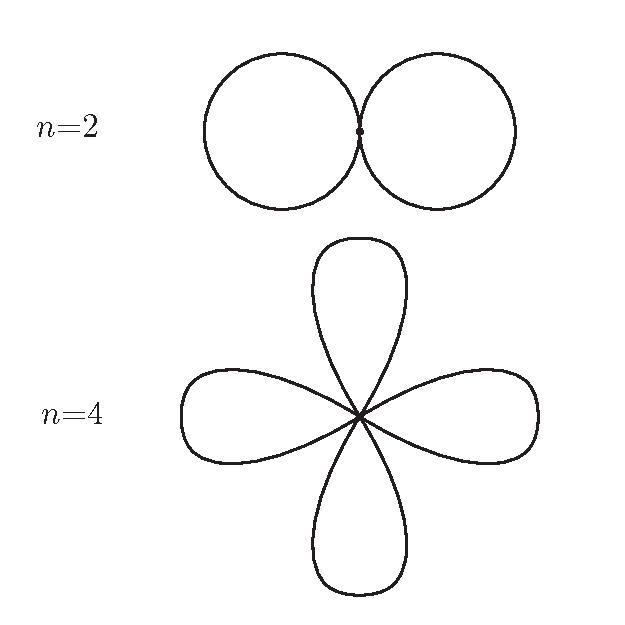
\includegraphics[trim=0cm 0cm 0cm 0cm,clip,scale=0.75]{images/bouquet.pdf}
\end{center}
\vspace{-8mm}
\end{define}
\begin{examples}\textsc{Altri esempi di equivalenze omotopiche.}
	\begin{enumerate}
		\item $\realset^2\setminus\left\{2\text{ punti}\right\}$ ha lo stesso tipo di omotopia di un \textit{bouquet di due circonferenze}: si può ottenere attraverso una composizione (continua) di retrazioni \textit{radiali} e \textit{lineari}.
		\begin{center}
						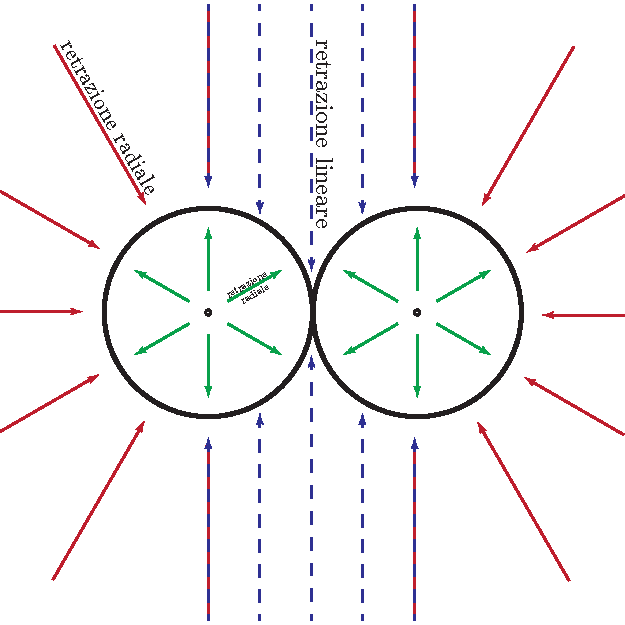
\includegraphics[trim=0cm 0cm 0cm 0cm,clip,scale=0.75]{images/bouquetconstruction.pdf}
		\end{center}	
		\item $\realset^2\setminus\left\{n\text{ punti}\right\}$ ha lo stesso tipo di omotopia di un \textit{bouquet di} $n$ \textit{circonferenze}.
		\item $\realset^3\setminus\left\{1\text{ retta}\right\}$ ha lo stesso tipo di omotopia di $\realset^2\setminus\left\{1\text{ punto}\right\}$ per retrazioni lineari, dunque ha la stessa omotopia di $S^1$ per i ragionamenti precedenti.
		\item Per $\realset^3\setminus\left\{2\text{ rette}\right\}$ dobbiamo distinguere a seconda della relazione fra le due rette.
		\begin{itemize}
			\item Se le rette sono \textbf{disgiunte}, $X$ è sempre omeomorfo a:
			\begin{equation*}
				\realset^3\setminus\left\{\text{asse z}\right\}\setminus\left\{x=y=1\right\}=\widetilde{X}
			\end{equation*}
		Cioè lo spazio $\realset^3$ privato di due rette perpendicolari al piano e distinte.\\
			Considerato ora il piano $Y=\left\{\text{piano xy}\right\}\setminus\left\{\left(0,0\right),\ \left(1,1\right)\right\}$, questo risulta un retratto di deformazione di $\widetilde{X}$ con retrazione:
			\begin{equation*}
				\funztot{r}{\widetilde{X}}{Y}{\left(x,\ y,\ z\right)}{\left(x,\ y, 0\right)}
			\end{equation*}
		Infatti la funzione è sempre ben definita e continua e, considerata la restrizione di $r$ ad $Y$, segue che banalmente che è l'identità di $Y$ in quanto tutti i punti di $Y$ hanno già la forma $\left(x,\ y, 0\right)$. Guardando invece $\widetilde{r}=i\circ r$ con $\incl{i}{Y}{\widetilde{X}}$, un'omotopia con $Id_{\widetilde{X}}$ è:
		\begin{equation*}
			\funz{F}{\widetilde{X}\times I}{\widetilde{X}}\ \colon \mvf{F}{\left(x,\ y,\ z\right)}{t}=\left(x,\ y,\ tz\right)
		\end{equation*}
		Infatti $F$ è banalmente ben definita continua, con $\mvf{F}{\mathbf{x}}{0}=\left(x,\ y,\ 0\right)=\widetilde{r}\left(\mathbf{x}\right)$ e $\mvf{F}{\mathbf{x}}{1}=\left(x,\ y,\ z\right)=Id_{\widetilde{X}}\left(\mathbf{x}\right)$.\\
		Segue che $\widetilde{X}$, e dunque anche $X$ per omeomorfismo, ha la stessa omotopia di $\realset^2\setminus\left\{2\text{ punti}\right\}$ e di un \textit{bouquet di due circonferenze}.
		\item Se le due rette sono \textbf{incidenti}, a meno di omeomorfismi si intersecano nell'origine. Consideriamo dunque $X=\realset^3\left\{r_1\cup r_2\right\}$ e lo spazio $A=S^2\setminus\left\{P_1,\ P_2,\ Q_1,\ Q_2\right\}$. Se prendiamo la retrazione:
		\begin{equation*}
			\funztot{r}{X}{A}{\mathbf{x}}{\frac{\mathbf{x}}{\labs \mathbf{x}\rabs}}.
		\end{equation*}
		e l'omotopia:
		\begin{equation*}
			\widetilde{r}\coloneqq\funztot{ i\circ r}{X}{X}{\mathbf{x}}{\frac{\mathbf{x}}{\labs \mathbf{x}\rabs}}
		\end{equation*}
	Si verifica in modo analogo a come visto nel caso della sfera e dello spazio privato dell'origine (esempio a pagina \ref{retrattosfera}), trattando con una \textit{retrazione radiale} ben definita e la sua omotopia nota, che $A$ è retratto di deformazione di $X$. Segue allora che hanno lo stesso tipo di omotopia.
		\end{itemize}
	\end{enumerate}
	\vspace{-3mm}
\end{examples}